\documentclass[11pt,aspectratio=169]{beamer}

% 直接复用现有主题配置。
% 通用宏包集中在此处；课程内容文件中通常不应再加载宏包。
\usepackage{iftex}
\ifPDFTeX
  \usepackage[T1]{fontenc}
  \usepackage[utf8]{inputenc}
  \usepackage{lmodern}
\else
  \usepackage{fontspec}
  \defaultfontfeatures{Ligatures=TeX}
\fi

\usepackage{amsmath,amssymb,mathtools}
\usepackage{booktabs}
\usepackage{graphicx}
\usepackage{tikz}
\usetikzlibrary{arrows.meta,positioning,shapes.geometric}
\usepackage[most]{tcolorbox}
\usepackage{listings}
\usepackage{xparse}
\usepackage{appendixnumberbeamer}
\usepackage[backend=biber,style=authoryear,maxcitenames=2]{biblatex}
% 修改整套课件配色时，只需要编辑本文件。
\definecolor{Primary}{HTML}{003B6F}
\definecolor{PrimaryLight}{HTML}{EAF2F8}
\definecolor{Accent}{HTML}{D97706}
\definecolor{AccentLight}{HTML}{FFF4E5}
\definecolor{Background}{HTML}{FFFFFF}
\definecolor{Text}{HTML}{20252B}
\definecolor{MutedText}{HTML}{66717E}
\definecolor{RuleColor}{HTML}{D7DEE5}
\definecolor{Success}{HTML}{237A57}
\definecolor{SuccessLight}{HTML}{EAF6F0}
\definecolor{CodeBackground}{HTML}{F5F7F9}
% 字体语义集中定义，避免在每一页手动设置字号与字重。
\ifPDFTeX
  \usefonttheme{professionalfonts}
\else
  \IfFontExistsTF{TeX Gyre Heros}{
    \setsansfont{TeX Gyre Heros}
  }{
    \setsansfont{Latin Modern Sans}
  }
  % TeX Gyre Cursor 随常见 TeX Live 安装提供，适合作为可移植的代码字体。
  \setmonofont{TeX Gyre Cursor}
\fi

\newcommand{\TitleFont}{\fontsize{25}{30}\selectfont\bfseries}
\newcommand{\SubtitleFont}{\large}
\newcommand{\FrameTitleFont}{\large\bfseries}
\newcommand{\BodyFont}{\normalsize}
\newcommand{\SmallFont}{\small}
\newcommand{\CodeFont}{\ttfamily\small}
% Beamer 外观：白底、蓝色主色、无导航按钮、极简页脚。
\mode<presentation>

\useinnertheme{rectangles}
\usefonttheme{professionalfonts}
\setbeamertemplate{navigation symbols}{}
\setbeamertemplate{headline}{}
\setbeamersize{text margin left=0.75cm,text margin right=0.75cm}

\setbeamercolor{normal text}{fg=Text,bg=Background}
\setbeamercolor{structure}{fg=Primary}
\setbeamercolor{alerted text}{fg=Accent}
\setbeamercolor{frametitle}{fg=Primary,bg=Background}
\setbeamercolor{title}{fg=Primary}
\setbeamercolor{subtitle}{fg=MutedText}
\setbeamercolor{author}{fg=Text}
\setbeamercolor{institute}{fg=MutedText}
\setbeamercolor{date}{fg=MutedText}
\setbeamercolor{itemize item}{fg=Primary}
\setbeamercolor{itemize subitem}{fg=Accent}
\setbeamercolor{section in toc}{fg=Text}
\setbeamercolor{section in toc shaded}{fg=MutedText}

\setbeamerfont{frametitle}{series=\bfseries,size=\large}
\setbeamerfont{title}{series=\bfseries,size=\LARGE}
\setbeamerfont{footline}{size=\scriptsize}

\setbeamertemplate{frametitle}{%
  \vspace{0.18cm}%
  \insertframetitle\par
  \vspace{0.10cm}%
  {\color{RuleColor}\rule{\textwidth}{0.5pt}}%
}

\setbeamertemplate{footline}{%
  \leavevmode
  \hbox{%
    \begin{beamercolorbox}[wd=.78\paperwidth,ht=2.8ex,dp=1.2ex,leftskip=.75cm]{normal text}%
      \color{MutedText}\insertshorttitle\enspace |\enspace\insertshortauthor
    \end{beamercolorbox}%
    \begin{beamercolorbox}[wd=.22\paperwidth,ht=2.8ex,dp=1.2ex,rightskip=.75cm plus1fil]{normal text}%
      \hfill\color{MutedText}\insertframenumber\,/\,\inserttotalframenumber
    \end{beamercolorbox}%
  }
}

\setbeamertemplate{title page}{%
  \vfill
  {\color{Primary}\rule{1.2cm}{3pt}\par}
  \vspace{0.55cm}
  {\TitleFont\color{Primary}\inserttitle\par}
  \vspace{0.18cm}
  {\SubtitleFont\color{MutedText}\insertsubtitle\par}
  \vspace{0.9cm}
  {\BodyFont\insertauthor\par}
  {\SmallFont\color{MutedText}\insertinstitute\par}
  \vspace{0.35cm}
  {\SmallFont\color{MutedText}\insertdate\par}
  \vfill
}

\setbeamertemplate{section page}{%
  \vfill
  {\color{MutedText}\large Chapter \insertsectionnumber\par}
  \vspace{0.25cm}
  {\color{Primary}\rule{1.2cm}{3pt}\par}
  \vspace{0.45cm}
  {\fontsize{27}{32}\selectfont\bfseries\color{Primary}\insertsectionhead\par}
  \vfill
}

\AtBeginSection[]{
  \begin{frame}[plain,noframenumbering]
    \sectionpage
  \end{frame}
}

\mode<all>
% 页面级语义环境。正文优先使用这些环境，而不是直接使用 frame。
\newenvironment{titleframe}
  {\begin{frame}[plain,noframenumbering]\titlepage}
  {\end{frame}}

\newenvironment{outlineframe}[1][Outline]
  {\begin{frame}{#1}\tableofcontents[currentsection,hideothersubsections]}
  {\end{frame}}

\newenvironment{theoryframe}[1]
  {\begin{frame}{#1}}
  {\end{frame}}

\newenvironment{exampleframe}[1]
  {\begin{frame}{#1}}
  {\end{frame}}

\newenvironment{figureframe}[1]
  {\begin{frame}{#1}\centering}
  {\end{frame}}

% fragile 页面必须通过 environment=codeframe 告知 Beamer 外层环境名。
\newenvironment{codeframe}[1]
  {\begin{frame}[fragile,environment=codeframe]{#1}}
  {\end{frame}}

\newenvironment{summaryframe}[1][Summary]
  {\begin{frame}{#1}}
  {\end{frame}}

\newcommand{\figurecaption}[1]{%
  \par\vspace{0.35cm}{\small\color{MutedText}#1\par}%
}
% 内容组件：信息框、强调命令、代码样式与常用数学命令。
\tcbset{
  coursebox/.style={
    enhanced,
    boxrule=0pt,
    leftrule=2.5pt,
    arc=1pt,
    outer arc=1pt,
    left=7pt,right=7pt,top=6pt,bottom=6pt,
    fonttitle=\bfseries,
    before skip=6pt,after skip=6pt
  }
}

\newtcolorbox{definitionbox}[1][Definition]{
  coursebox,title=#1,colback=PrimaryLight,colframe=Primary,coltitle=Primary
}
\newtcolorbox{theorembox}[1][Theorem]{
  coursebox,title=#1,colback=PrimaryLight,colframe=Primary,coltitle=Primary
}
\newtcolorbox{proofbox}[1][Proof idea]{
  coursebox,title=#1,colback=SuccessLight,colframe=Success,coltitle=Success
}
\newtcolorbox{remarkbox}[1][Remark]{
  coursebox,title=#1,colback=CodeBackground,colframe=MutedText,coltitle=Text
}
\newtcolorbox{warningbox}[1][Warning]{
  coursebox,title=#1,colback=AccentLight,colframe=Accent,coltitle=Accent
}
\newtcolorbox{importantbox}[1][Important]{
  coursebox,title=#1,colback=AccentLight,colframe=Accent,coltitle=Accent
}

\newcommand{\keyterm}[1]{\textcolor{Primary}{\textbf{#1}}}
\newcommand{\coursecheck}{\textcolor{Success}{\ensuremath{\checkmark}}}

\lstdefinestyle{coursecode}{
  basicstyle=\CodeFont,
  backgroundcolor=\color{CodeBackground},
  keywordstyle=\color{Primary}\bfseries,
  commentstyle=\color{Success},
  stringstyle=\color{Accent},
  numbers=left,
  numberstyle=\tiny\color{MutedText},
  numbersep=8pt,
  frame=single,
  rulecolor=\color{RuleColor},
  framesep=7pt,
  showstringspaces=false,
  breaklines=true,
  columns=fullflexible,
  keepspaces=true,
  tabsize=2
}
\lstset{style=coursecode}

\newcommand{\R}{\mathbb{R}}
\newcommand{\N}{\mathbb{N}}

\addbibresource{../Causal_Inference_C/Beamer/Reference list/bibliography.bib}

% 课程信息：以后通常只需要修改这里和正文内容。
\title[Causal Inference]{Causal Inference}
\subtitle{Potential Outcome Framework}
\author[Zhaoyi]{Zhaoyi}
%\institute[Your University]{Your University}
\date{\today}

\begin{document}

\begin{titleframe}


\end{titleframe}


\begin{outlineframe}

\end{outlineframe}
\section{Potential Outcome Framework}

\begin{frame}{Framework: Brainstorm}


\end{frame}


\begin{frame}
\subsection*{Treatment Allocation and Outcomes}

\textbf{Example: Hospital Visit and Health}
\begin{itemize}
    \item Consider a single individual $i$
    \item Outcome: $Y_i = \text{future health status}$
    \item Treatment: $D_i = \text{went to the hospital}$
\end{itemize}

$$D_i = \begin{cases} 
1, & \text{if } i \text{ went to the hospital (treated)} \\ 
0, & \text{if } i \text{ did not (control)} 
\end{cases}$$

The empirical difficulty is that hospital attendance is typically endogenous: patients select into treatment based on symptoms, perceived severity, access, and physician advice.
\end{frame}

\begin{frame}

\subsection*{Potential Outcomes}

\textbf{Idea: Think of two parallel worlds}
\begin{itemize}
    \item Hospital example:
    \begin{itemize}
        \item[\blacksquare] $Y_i(1)$: health if person $i$ goes to the hospital
        \item[\blacksquare] $Y_i(0)$: health if person $i$ does not go
    \end{itemize}
    \item General definition:
    $$Y_i(1) : \text{outcome if treated}$$
    $$Y_i(0) : \text{outcome if not treated (control)}$$
    \item Both refer to the same individual in two alternative scenarios; it is not a before/after comparison.
    \item Fundamental problem: We only observe one of the two outcomes and the other is \textbf{counterfactual}.
\end{itemize}

\end{frame}
\begin{frame}

\subsection*{Realized Outcomes}

\begin{itemize}
    \item The outcome $Y_i$ is observed, which is a function of the potential outcomes and the treatment:
    $$Y_i = D_iY_i(1) + (1 - D_i)Y_i(0)$$
    $$= Y_i(0) + [Y_i(1) - Y_i(0)]D_i$$
    \item We observe the treated outcome if treated, otherwise the control outcome.
    \item Hospital example: Observed data show the patient's health only under the realized treatment; the counterfactual outcome is unobserved.
    \item Sometimes referred to as the \textbf{switching equation}.
    \item Extensions to multiple or continuous treatments are possible and discussed in the literature, but beyond the scope of this course.
\end{itemize}

\end{frame}


\begin{frame}{}
Let me put numbers on this, because I think the sign of what happens is genuinely surprising. 
Take a hospital. The treatment is going to hospital, and the outcome is a health score, where higher means healthier. 
Ten people. Four of them go to hospital, six don't. And the people who go are the ones who feel sick, which is the whole point.

\begin{center}
\begin{tabular}{lcccc}
\hline
& $n$ & $Y(0)$ & $Y(1)$ & observed \\
\hline
Went to hospital ($D=1$) & 4 & 2 & 5 & 5 \\
Stayed home ($D=0$) & 6 & 6 & 9 & 6 \\
\hline
\end{tabular}
\end{center}

We can see, if we choose the naive comparison, the difference is 1. But this is not causal effect if we don't add any assumptions. We will see it later.

\end{frame}




\section{Stable Unit Treatment Value Assumption (SUTVA)}

\begin{frame}{Why SUTVA Matters}


In the most general case, unit $i$'s outcome may depend on the entire treatment assignment vector:
$$Y_i(D_1, \dots, D_N) = Y_i(D).$$

These are $2^N$ potential outcomes!

This allows for:
\begin{itemize}
    \item \textbf{interference}: other units' treatment affects unit $i$'s outcome;
    \item \textbf{different versions of treatment}: the same treatment label may correspond to different interventions.
\end{itemize}

To simplify the analysis, we often impose \textbf{SUTVA}.
\end{frame}


\begin{frame}{Stable Unit Treatment Value Assumption (SUTVA)}


\begin{enumerate}
    \item \textbf{No interference:}
    $$Y_i(D) = Y_i(D_i),$$
    so unit $i$'s potential outcome depends only on its own treatment.
    \item \textbf{Consistency / no hidden versions of treatment:} if $D_i = d$, then
    $$Y_i = Y_i(d).$$
\end{enumerate}

Under SUTVA, we can write potential outcomes simply as $Y_i(1)$ and $Y_i(0)$.


\end{frame}

\begin{frame}{When Can SUTVA Fail?}

SUTVA may be violated when units affect one another.

Examples include:
\begin{itemize}
    \item \textbf{social interactions or contagion} between individuals;
    \item \textbf{spillovers} across firms, schools, or regions;
    \item \textbf{equilibrium effects}, where treatment changes market-wide outcomes.
\end{itemize}

Suppose treatment is hospital admission.
\begin{itemize}
    \item Under SUTVA, patient $i$'s future health depends only on whether patient $i$ is admitted.
    \item SUTVA would fail if patient $i$'s outcome also depends on whether many other patients are admitted, e.g., because hospital congestion affects quality of care.
\end{itemize}
\end{frame}


\section{Treatment Effects: Naive Comparison and Selection Bias}

\begin{frame}
I will use another screen to explain the setting and the problem we face, so does the proof.

Then I will introduce the "Selection Bias".
\end{frame}



\section{Identification(Practice)}

\begin{frame}{Independence Assumption}

\textbf{Assumption: Random Assignment}
\begin{theorembox}
Suppose that the treatement variable is independent from the potential outcome, we have such notation:$$(Y_i(1),Y_i(0))\perp D_i$$
\end{theorembox}

Next Step, we can have some theroems under random assignment

\end{frame}
\begin{frame}
\textbf{Theorem: ATE}
Under random assignment, it holds that 
\begin{theorembox}
$$E[Y_i\vert D=1]-E[Y_i\vert D=0] =\tau_{ATE}=\tau_{ATET}=\tau_{ATEU}$$

\end{theorembox}


\end{frame}


\begin{frame}{What other things should we pay attention to?}
\begin{itemize}
     
    \item The ATE provides only a limited summary of the treatment effect.
    \begin{itemize}
        \item If treatment effects vary across individuals, two groups can have the same mean but very different distributions—for example, the same average income but different levels of inequality or tail behavior.
    \end{itemize}
        \item Policy relevance: We may care more about the impact on specific \textbf{subgroups}.
    \begin{itemize}
        \item Does the treatment benefit the most disadvantaged?
        \item Are some individuals harmed?
    \end{itemize}
        \item We will see that these questions are generally difficult to answer, but we discuss two parameters that aim to address them: distributional and quantile treatment effects.
\end{itemize}


\end{frame}

\begin{frame}{Distribution Treatment Effects}

The distribution treatment effect of $y \in \mathbb{R}$ is defined as
$$\tau_{DTE}(y) = F_{Y(1)}(y) - F_{Y(0)}(y).$$

\textbf{Proposition: DTE}
Under random assignment, $\tau_{DTE}(y)$ is identified for all $y \in \mathbb{R}$.

\end{frame}


\begin{frame}{Quantile Treatment Effects}

Suppose that $Y_i(d)$ is a continuous random variable and $Q_{Y(d)}$ be the quantile function of $Y_i(d)$ for $d \in \{0, 1\}$.

The \emph{quantile treatment effect} for quantile $\tau$ is given by
$$\tau_{QTE}(\delta) \equiv Q_{Y(1)}(\delta) - Q_{Y(0)}(\delta).$$

\textbf{Proposition: QTE}
Under random assignment, $\tau_{QTE}(\delta)$ is identified for all quantile $\delta \in (0, 1)$.

\end{frame}

\begin{frame}{Quantile Treatment Effects (QTE)}

\begin{itemize}
    \item It may be tempting to interpret $\tau_{QTE}(\delta)$ as the $\delta$-th of the distribution of individual treatment effects, for example, the median of $\tau_i = Y_i(1) - Y_i(0)$.
    \item However, this interpretation is generally incorrect, as the quantile of a difference $\neq$ the difference of quantiles.
\end{itemize}

\textbf{Example}
Let $Y_i(0) \sim \mathcal{N}(0, 1)$ and $Y_i(1) = -Y_i(0)$.
Then $Q_{Y(1)}(\delta) - Q_{Y(0)}(\delta) = 0$ for all $\delta$, but $Q_{Y(1)-Y(0)}(\delta) \neq 0$ for all $\delta \neq 0.5$

$$\implies \text{the quantile of the difference of the potential outcomes is not equal to the difference}$$
$$\text{of quantiles of the potential outcomes in general.}$$

\end{frame}


\begin{frame}


\end{frame}


\section{Directed Acyclic Graphs}
\begin{frame}{Potential Outcomes and DAGs}

\begin{itemize}
    \item So far, we have used the potential outcomes framework to define causal effects through counterfactuals.
    \item DAGs provide a complementary graphical language for causal reasoning.
    \item Potential outcomes ask: \emph{What would happen to $Y$ if we set $D = 1$ rather than $D = 0$?}
    \item DAGs ask: \emph{How are variables causally related?}
    \item DAGs make assumptions about causal structure explicit, including:
    \begin{itemize}
        \item[\blacksquare] which variables affect each other
        \item[\blacksquare] where confounding comes from
        \item[\blacksquare] what it means to intervene on treatment
    \end{itemize}
    \item In this course, DAGs are mainly a tool for intuition and for thinking about identification.
\end{itemize}

\end{frame}

\begin{frame}[label=dag-layout]{Directed Acyclic Graphs (DAGs)}

\begin{columns}[c,onlytextwidth]
\begin{column}{0.57\textwidth}
\small

A DAG represents causal relationships between variables.

\begin{itemize}
    \item \textbf{Nodes:} variables (e.g. $D, X, Y, U$)
    \item \textbf{Arrows:} direct causal effects
    \item \textbf{Directed:} arrows have a direction
    \item \textbf{Acyclic:} no directed feedback loops
    \item A DAG is a model, not the data
\end{itemize}

DAGs help us state assumptions explicitly and reason about identification.
\end{column}
\begin{column}{0.39\textwidth}
\centering
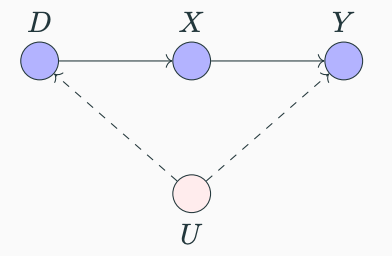
\includegraphics[width=\linewidth,height=0.65\textheight,keepaspectratio]{Courses/image_2.png}
\end{column}
\end{columns}
\end{frame}

\begin{frame}{Example: Smoking and Lung Cancer}

Variables:

\begin{columns}[c,onlytextwidth]
\begin{column}{0.57\textwidth}
\small
\begin{itemize}
    \item $D$: smoking
    \item $Y$: lung cancer
    \item $X$: tar deposits
    \item $U$: unobserved predisposition
\end{itemize}

Interpretation:
\begin{itemize}
    \item Smoking increases tar deposits
    \item Tar deposits increase lung cancer risk
    \item $U$ affects both smoking and lung cancer
    \item $X$ is a mediator
    \item $U$ is an unobserved confounder
\end{itemize}
\end{column}
\begin{column}{0.39\textwidth}
\centering

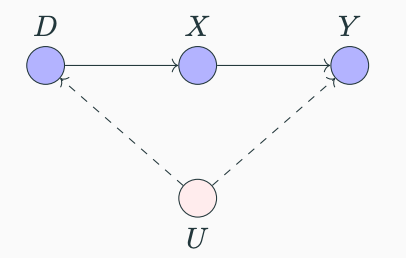
\includegraphics[width=1\textwidth]{Courses/image_3.png}
\end{column}
\end{columns}
\end{frame}


\begin{frame}{What the Graph Tells Us}

\begin{itemize}
    \item The graph encodes:
    $$D \to X \to Y, \quad U \to D, \quad U \to Y$$
    \item Smoking affects lung cancer through tar deposits.
    \item Smoking and lung cancer also share a common cause $U$.
    \item So the observed association between $D$ and $Y$ need not equal the causal effect.
\end{itemize}
\end{frame}


\begin{frame}{The do-Operator}
\begin{columns}[c,onlytextwidth]
\begin{column}{0.57\textwidth}
\small
\begin{itemize}
    \item $\text{do}(D = d)$ means we externally set treatment to $d$.
    \item Graphically, this removes all incoming arrows into $D$.
    \item In particular, $U$ no longer affects treatment assignment.
    \item The intervention distribution is
    $$f_{Y \mid \text{do}(D=d)}(y).$$
\end{itemize}
\end{column}
\begin{column}{0.39\textwidth}
\centering

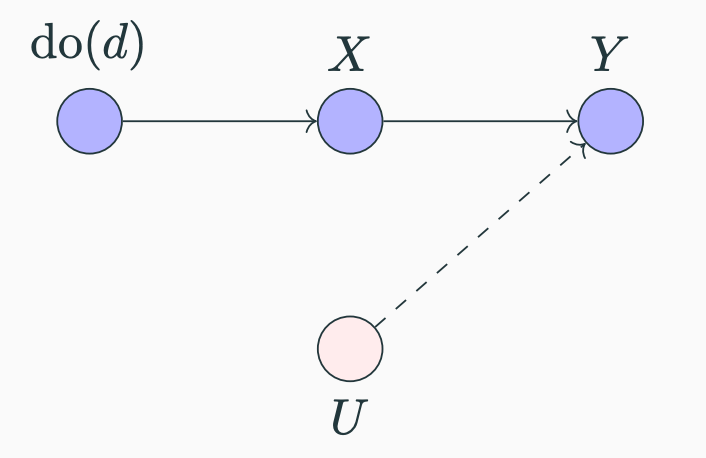
\includegraphics[width=0.9\textwidth]{Courses/image_4.png}

\end{column}
\end{columns}

\end{frame}
\section{Key Takeaways}








\begin{frame}{Key Takeaways}

\begin{itemize}
    \item We know the basic framework of potential outcome.
    \item SUTVA is a crucial assmption
    \item Naive Comparison is not that convincing, so if we could construct the assumptions, we can exclude the "selection bias". Therefore, we could know ATE under "random assignment".
    \item Identification tells us if we could observe outcomes from population (sample...)
    \item Short explain the DAG, useful tool while doing a research.
\end{itemize}


\end{frame}



\begin{frame}{Next Step}
\begin{importantbox}
Next lecture we will explore the topic "Randomized Experiment". 
\end{importantbox}
\end{frame}


\begin{frame}[allowframebreaks]{References}
    \small
    \nocite{CunninghamScott2021Ci:t,wager2024causal}
    \printbibliography[heading=none]
\end{frame}



\end{document}